\documentclass[tikz,border=0pt]{standalone}
\usepackage{xcolor}
\usetikzlibrary{calc}
% Palette: Sam_Comm_final.png by eye, and the drones and raiders.
\definecolor{ink}{HTML}{3B2340}
\definecolor{sky}{HTML}{EFC46A}
\definecolor{skyhi}{HTML}{F5DA92}
\definecolor{skylow}{HTML}{E9B060}
\definecolor{cloud}{HTML}{F2D58A}
\definecolor{paper}{HTML}{FBEFD0}
\definecolor{cream}{HTML}{FFF6E0}
\definecolor{white}{HTML}{FFFFFF}
\definecolor{wallA}{HTML}{E88A73}
\definecolor{wallB}{HTML}{EE9F7E}
\definecolor{wallC}{HTML}{E47A7E}
\definecolor{wallD}{HTML}{F0B07E}
\definecolor{wallE}{HTML}{D9765F}
\definecolor{wallF}{HTML}{E99A8A}
\definecolor{greenA}{HTML}{8DBB7E}
\definecolor{greenB}{HTML}{6FA77A}
\definecolor{greenC}{HTML}{A9C97F}
\definecolor{greenD}{HTML}{5E9C6A}
\definecolor{greenE}{HTML}{4A8060}
\definecolor{sage}{HTML}{9DB98A}
\definecolor{sagedark}{HTML}{6F8F66}
\definecolor{sagelight}{HTML}{C2D6A6}
\definecolor{window}{HTML}{F6E7A0}
\definecolor{windark}{HTML}{8C5A64}
\definecolor{metal}{HTML}{8D9A93}
\definecolor{metaldark}{HTML}{5E6B66}
\definecolor{metallight}{HTML}{B9C4BC}
\definecolor{wood}{HTML}{B9835A}
\definecolor{wooddark}{HTML}{8C5A3C}
\definecolor{woodlight}{HTML}{D9A66F}
\definecolor{stone}{HTML}{E7C9A0}
\definecolor{stonedark}{HTML}{C9A47E}
\definecolor{concrete}{HTML}{D8C3A4}
\definecolor{concretedark}{HTML}{B8A084}
\definecolor{asphalt}{HTML}{8E7A86}
\definecolor{asphaltdark}{HTML}{6E5C68}
\definecolor{roadline}{HTML}{F6E7A0}
\definecolor{kerb}{HTML}{D8B48C}
\definecolor{red}{HTML}{E0483E}
\definecolor{redlight}{HTML}{F27A6A}
\definecolor{gold}{HTML}{FFB000}
\definecolor{goldlight}{HTML}{FFD54F}
\definecolor{teal}{HTML}{4FA3A0}
\definecolor{tealdark}{HTML}{3C8582}
\definecolor{magenta}{HTML}{FF2E88}
\definecolor{cyan}{HTML}{13CFE3}
\definecolor{violet}{HTML}{8A5BD6}
\definecolor{orange}{HTML}{F2803A}
\definecolor{pink}{HTML}{F48FB1}
\definecolor{glow}{HTML}{4FE6E0}
\definecolor{glowhi}{HTML}{C8FFF9}
\definecolor{hot}{HTML}{FF6A1A}
\definecolor{hothi}{HTML}{FFD07A}
\definecolor{armour}{HTML}{7E7A86}
\definecolor{armourdark}{HTML}{5A5466}
\definecolor{armourlight}{HTML}{A8A2B0}
\definecolor{wasp}{HTML}{E0A82E}
\definecolor{waspdark}{HTML}{B07E1A}
\definecolor{moth}{HTML}{F2E6C8}
\definecolor{mothdark}{HTML}{D2C09A}
\definecolor{hornet}{HTML}{3C8582}
\definecolor{hornetdark}{HTML}{2C6260}
\definecolor{warden}{HTML}{E47A7E}
\definecolor{wardendark}{HTML}{B85A62}
\definecolor{tick}{HTML}{8DBB7E}
\definecolor{tickdark}{HTML}{5E8A5A}
\definecolor{strider}{HTML}{D9765F}
\definecolor{striderdark}{HTML}{A8543F}
\definecolor{jacket}{HTML}{6FA77A}
\definecolor{jacketb}{HTML}{4FA3A0}
\definecolor{jacketc}{HTML}{E88A73}
\definecolor{jacketd}{HTML}{F0B07E}
\definecolor{skin}{HTML}{F2C49A}
\definecolor{skinb}{HTML}{C98C6A}
\definecolor{skinc}{HTML}{8C5A3C}
\definecolor{hair}{HTML}{3B2340}
\definecolor{goo}{HTML}{B6E35A}
\definecolor{goodark}{HTML}{7FB23A}
\newcommand{\Ink}{1.8pt}
\tikzset{inked/.style={draw=ink, line width=\Ink, line join=round, line cap=round}}
\begin{document}
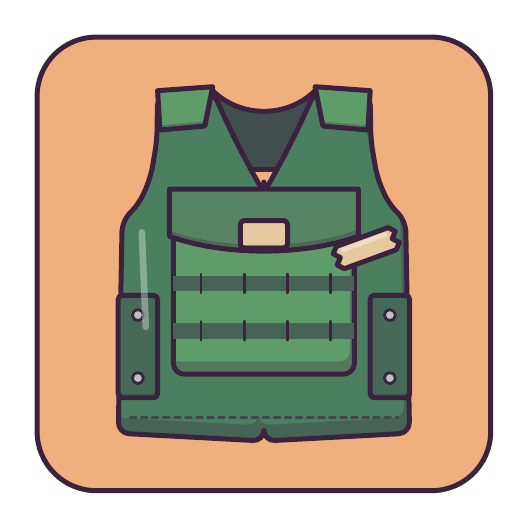
\begin{tikzpicture}
\clip (0,0) rectangle (6,6);
\fill[wallD] [rounded corners=0.75cm] (0.12,0.12) rectangle (5.88,5.88);
\begin{scope}\clip [rounded corners=0.75cm] (0.12,0.12) rectangle (5.88,5.88);
\filldraw[inked, fill=greenE!45!ink] (2.35,5.2) .. controls (2.7,4.85) and (3.3,4.85) .. (3.65,5.2) -- (3.3,4.2) -- (2.7,4.2) -- cycle;
\begin{scope}\clip [rounded corners=0.14cm] (3,3.9) -- (3.191,4.244) -- (3.363,4.575) -- (3.516,4.894) -- (3.65,5.2) -- (4.35,5.15) -- (4.359,4.562) -- (4.438,4.1) -- (4.584,3.763) -- (4.8,3.55) -- (4.85,0.85) -- (3,0.75) -- (3,0.75) -- (1.15,0.85) -- (1.2,3.55) -- (1.416,3.763) -- (1.562,4.1) -- (1.641,4.562) -- (1.65,5.15) -- (2.35,5.2) -- (2.484,4.894) -- (2.637,4.575) -- (2.809,4.244) -- (3,3.9) -- cycle;
\fill[greenE!70!ink] [rounded corners=0.14cm] (3,3.9) -- (3.191,4.244) -- (3.363,4.575) -- (3.516,4.894) -- (3.65,5.2) -- (4.35,5.15) -- (4.359,4.562) -- (4.438,4.1) -- (4.584,3.763) -- (4.8,3.55) -- (4.85,0.85) -- (3,0.75) -- (3,0.75) -- (1.15,0.85) -- (1.2,3.55) -- (1.416,3.763) -- (1.562,4.1) -- (1.641,4.562) -- (1.65,5.15) -- (2.35,5.2) -- (2.484,4.894) -- (2.637,4.575) -- (2.809,4.244) -- (3,3.9) -- cycle;
\fill[greenE, shift={(-0.07,0.2)}] [rounded corners=0.14cm] (3,3.9) -- (3.191,4.244) -- (3.363,4.575) -- (3.516,4.894) -- (3.65,5.2) -- (4.35,5.15) -- (4.359,4.562) -- (4.438,4.1) -- (4.584,3.763) -- (4.8,3.55) -- (4.85,0.85) -- (3,0.75) -- (3,0.75) -- (1.15,0.85) -- (1.2,3.55) -- (1.416,3.763) -- (1.562,4.1) -- (1.641,4.562) -- (1.65,5.15) -- (2.35,5.2) -- (2.484,4.894) -- (2.637,4.575) -- (2.809,4.244) -- (3,3.9) -- cycle;
\end{scope}
\draw[inked] [rounded corners=0.14cm] (3,3.9) -- (3.191,4.244) -- (3.363,4.575) -- (3.516,4.894) -- (3.65,5.2) -- (4.35,5.15) -- (4.359,4.562) -- (4.438,4.1) -- (4.584,3.763) -- (4.8,3.55) -- (4.85,0.85) -- (3,0.75) -- (3,0.75) -- (1.15,0.85) -- (1.2,3.55) -- (1.416,3.763) -- (1.562,4.1) -- (1.641,4.562) -- (1.65,5.15) -- (2.35,5.2) -- (2.484,4.894) -- (2.637,4.575) -- (2.809,4.244) -- (3,3.9) -- cycle;
\begin{scope}\clip (2.35,5.25) -- (1.65,5.2) -- (1.68,4.7) -- (2.25,4.75) -- cycle;
\fill[greenD!70!ink] (2.35,5.25) -- (1.65,5.2) -- (1.68,4.7) -- (2.25,4.75) -- cycle;
\fill[greenD, shift={(-0.021,0.06)}] (2.35,5.25) -- (1.65,5.2) -- (1.68,4.7) -- (2.25,4.75) -- cycle;
\end{scope}
\draw[inked] (2.35,5.25) -- (1.65,5.2) -- (1.68,4.7) -- (2.25,4.75) -- cycle;
\begin{scope}\clip (3.65,5.25) -- (4.35,5.2) -- (4.32,4.7) -- (3.75,4.75) -- cycle;
\fill[greenD!70!ink] (3.65,5.25) -- (4.35,5.2) -- (4.32,4.7) -- (3.75,4.75) -- cycle;
\fill[greenD, shift={(-0.021,0.06)}] (3.65,5.25) -- (4.35,5.2) -- (4.32,4.7) -- (3.75,4.75) -- cycle;
\end{scope}
\draw[inked] (3.65,5.25) -- (4.35,5.2) -- (4.32,4.7) -- (3.75,4.75) -- cycle;
\begin{scope}\clip[rounded corners=0.14cm] (1.85,1.6) rectangle (4.15,3.9);
\fill[greenD!70!ink,rounded corners=0.14cm] (1.85,1.6) rectangle (4.15,3.9);
\fill[greenD,rounded corners=0.14cm, shift={(-0.056,0.16)}] (1.85,1.6) rectangle (4.15,3.9);
\end{scope}
\draw[inked,rounded corners=0.14cm] (1.85,1.6) rectangle (4.15,3.9);
\begin{scope}\clip (1.8,3.95) -- (4.2,3.95) -- (4.2,3.35) .. controls (3.5,3.1) and (2.5,3.1) .. (1.8,3.35) -- cycle;
\fill[greenD!80!ink!70!ink] (1.8,3.95) -- (4.2,3.95) -- (4.2,3.35) .. controls (3.5,3.1) and (2.5,3.1) .. (1.8,3.35) -- cycle;
\fill[greenD!80!ink, shift={(-0.028,0.08)}] (1.8,3.95) -- (4.2,3.95) -- (4.2,3.35) .. controls (3.5,3.1) and (2.5,3.1) .. (1.8,3.35) -- cycle;
\end{scope}
\draw[inked] (1.8,3.95) -- (4.2,3.95) -- (4.2,3.35) .. controls (3.5,3.1) and (2.5,3.1) .. (1.8,3.35) -- cycle;
\begin{scope}\clip[rounded corners=0.05cm] (2.7,3.2) rectangle (3.3,3.55);
\fill[stone!70!ink,rounded corners=0.05cm] (2.7,3.2) rectangle (3.3,3.55);
\fill[stone,rounded corners=0.05cm, shift={(-0.014,0.04)}] (2.7,3.2) rectangle (3.3,3.55);
\end{scope}
\draw[inked,rounded corners=0.05cm] (2.7,3.2) rectangle (3.3,3.55);
\fill[greenE!70!ink] (1.85,2.05) rectangle (4.15,2.25);
\draw[ink, line width=1pt, line cap=round] (2.2,2.03) -- (2.2,2.27);
\draw[ink, line width=1pt, line cap=round] (2.75,2.03) -- (2.75,2.27);
\draw[ink, line width=1pt, line cap=round] (3.3,2.03) -- (3.3,2.27);
\draw[ink, line width=1pt, line cap=round] (3.85,2.03) -- (3.85,2.27);
\fill[greenE!70!ink] (1.85,2.65) rectangle (4.15,2.85);
\draw[ink, line width=1pt, line cap=round] (2.2,2.63) -- (2.2,2.87);
\draw[ink, line width=1pt, line cap=round] (2.75,2.63) -- (2.75,2.87);
\draw[ink, line width=1pt, line cap=round] (3.3,2.63) -- (3.3,2.87);
\draw[ink, line width=1pt, line cap=round] (3.85,2.63) -- (3.85,2.87);
\begin{scope}\clip[rounded corners=0.05cm] (1.15,1.3) rectangle (1.65,2.6);
\fill[greenE!75!ink!70!ink,rounded corners=0.05cm] (1.15,1.3) rectangle (1.65,2.6);
\fill[greenE!75!ink,rounded corners=0.05cm, shift={(-0.017,0.05)}] (1.15,1.3) rectangle (1.65,2.6);
\end{scope}
\draw[inked,rounded corners=0.05cm] (1.15,1.3) rectangle (1.65,2.6);
\filldraw[inked,fill=metallight,line width=1.0pt] (1.4,2.35) circle (0.07);
\filldraw[inked,fill=metallight,line width=1.0pt] (1.4,1.55) circle (0.07);
\begin{scope}\clip[rounded corners=0.05cm] (4.35,1.3) rectangle (4.85,2.6);
\fill[greenE!75!ink!70!ink,rounded corners=0.05cm] (4.35,1.3) rectangle (4.85,2.6);
\fill[greenE!75!ink,rounded corners=0.05cm, shift={(-0.017,0.05)}] (4.35,1.3) rectangle (4.85,2.6);
\end{scope}
\draw[inked,rounded corners=0.05cm] (4.35,1.3) rectangle (4.85,2.6);
\filldraw[inked,fill=metallight,line width=1.0pt] (4.6,2.35) circle (0.07);
\filldraw[inked,fill=metallight,line width=1.0pt] (4.6,1.55) circle (0.07);
\draw[greenE!40!ink, line width=0.9pt, line cap=round, dash pattern=on 2.2pt off 1.8pt] (1.3,1.05) -- (4.7,1.05);
\filldraw[inked,fill=stone] (4.022,2.939) -- (4.68,3.179) -- (4.72,3.273) -- (4.629,3.32) -- (4.669,3.414) -- (4.578,3.461) -- (3.92,3.221) -- (3.88,3.127) -- (3.971,3.08) -- (3.931,2.986) -- cycle;
\fill[white, opacity=0.35] (4.001,3.144) -- (4.565,3.35) -- (4.544,3.406) -- (3.98,3.201) -- cycle;
\draw[white, line width=2.4pt, line cap=round, line join=round, opacity=0.35] plot[smooth, tension=0.6] coordinates {(1.45,3.4) (1.5,2.2)};
\end{scope}
\draw[inked] [rounded corners=0.75cm] (0.12,0.12) rectangle (5.88,5.88);
\end{tikzpicture}
\end{document}
